%%%%%%%%%%%%%%%%%%%%%%%%%%%%%%%%%%%%%%%%%%%%%%%%%%%%%%%%%%%%%%%%%%%%%%%%%%%%%%

\documentclass[unknownkeysallowed,10pt,xcolor={dvipsnames}]{beamer}

%%%%%%%%%%%%%%%%%%%%%%%%%%%%%%%%%%%%%%%%%%%%%%%%%%%%%%%%%%%%%%%%%%%%%%%%%%%%%%

\usetheme{Boadilla}
%\usetheme{default}
\usefonttheme{serif}
\usecolortheme{default}

%%%%%%%%%%%%%%%%%%%%%%%%%%%%%%%%%%%%%%%%%%%%%%%%%%%%%%%%%%%%%%%%%%%%%%%%%%%%%%

%\usepackage{euler,palatino}
\usepackage{lmodern}
\usepackage{amsmath,amssymb}
\usepackage[utf8]{inputenc}
\usepackage{xxcolor}
\usepackage{graphicx}
\usepackage[ruled]{algorithm2e}
\usepackage[english]{babel}
\usepackage{rotate}
\usepackage{shuffle}
%\usepackage{minted}
\usepackage{url}
\usepackage{etoolbox}
\usepackage{tikz}
\usepackage{rotating}
\usetikzlibrary{snakes}
\usetikzlibrary{trees}
\usetikzlibrary{arrows}
\usetikzlibrary{matrix}
\usetikzlibrary{calc}

%%%%%%%%%%%%%%%%%%%%%%%%%%%%%%%%%%%%%%%%%%%%%%%%%%%%%%%%%%%%%%%%%%%%%%%%%%%%%%

\usepackage{csquotes}
\usepackage{breakcites}
\usepackage{hyperref}
\usepackage[autocite=superscript,
            sortcites,
            maxcitenames=3,
            doi=false,
            isbn=false,
            note=false,
            url=false,
            bibstyle=authoryear,
            style=authoryear,
            backend=bibtex]{biblatex}

\AtEveryCitekey{%
    \clearfield{title}%
    \clearfield{note}%
    \clearfield{pages}%
    \clearlist{location}%
    \clearlist{publisher}%
    \clearname{editor}%
}% end AtEveryCitekey

\bibliography{biblio.bib}
\renewcommand*{\multicitedelim}{\\}
\renewcommand{\footfullcite}[1]{\footnote[frame]{\fullcite{#1}}}
\def\bibfont{\tiny}
\beamertemplatenavigationsymbolsempty

% Affichage du plan à chaque changement de partie.
\AtBeginSection[]{
    \frame<handout:0>{
        \frametitle{Contents}
        \tableofcontents[
            sectionstyle=show/hide,
            subsectionstyle=show/shaded/hide]}
}

%%%%%%%%%%%%%%%%%%%%%%%%%%%%%%%%%%%%%%%%%%%%%%%%%%%%%%%%%%%%%%%%%%%%%%%%%%%%%%

\definecolor{Vert}{RGB}{20,100,20}
\setbeamercolor{title}{fg=Vert}
\setbeamercolor{frametitle}{fg=Vert}
\setbeamercolor{structure}{fg=Vert}

%%%%%%%%%%%%%%%%%%%%%%%%%%%%%%%%%%%%%%%%%%%%%%%%%%%%%%%%%%%%%%%%%%%%%%%%%%%%%%

\setbeamercovered{dynamic}

%%%%%%%%%%%%%%%%%%%%%%%%%%%%%%%%%%%%%%%%%%%%%%%%%%%%%%%%%%%%%%%%%%%%%%%%%%%%%%

\DeclareMathOperator{\QQ}{\mathbb{Q}}
\DeclareMathOperator{\STD}{\mathrm{std}}
\DeclareMathOperator{\SHUFFLE}{\bullet}
\DeclareMathOperator{\La}{\mathtt{a}}
\DeclareMathOperator{\Lb}{\mathtt{b}}

\newcommand{\BIB}[2]{{\footnotesize\textcolor{MidnightBlue!85}{[\textbf{#1}, #2]}}}

%%%%%%%%%%%%%%%%%%%%%%%%%%%%%%%%%%%%%%%%%%%%%%%%%%%%%%%%%%%%%%%%%%%%%%%%%%%%%%

\newcommand{\MWithContainment}{%
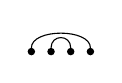
\begin{tikzpicture}[scale=0.1,inner sep=.8pt,node distance=.25cm]
\draw node [draw,circle,fill=black] (U1)               {};
\draw node [draw,circle,fill=black] [right of=U1] (U2) {};
\draw node [draw,circle,fill=black] [right of=U2] (U3) {};
\draw node [draw,circle,fill=black] [right of=U3] (U4) {};
\draw (U2.north) .. controls ($ (U2.north) + (0,1.75) $) and ($ (U3.north) + (0,1.75) $) .. (U3.north);
\draw (U1.north) .. controls ($ (U1.north) + (0,2.5) $) and ($ (U4.north) + (0,2.5) $) .. (U4.north);
\end{tikzpicture}
}% end \MWithContainment

\newcommand{\Crossing}{%
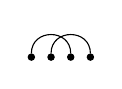
\begin{tikzpicture}[yscale=0.08,xscale=0.09,inner sep=.8pt,node distance=.25cm,>=latex']%,>=stealth',->]
\draw node [draw,circle,fill=black] (U1)               {};
\draw node [draw,circle,fill=black] [right of=U1] (U2) {};
\draw node [draw,circle,fill=black] [right of=U2] (U3) {};
\draw node [draw,circle,fill=black] [right of=U3] (U4) {};
\draw [] (U1.north) .. controls ($ (U1.north) + (0,4) $) and ($ (U3.north) + (0,4) $) .. (U3.north);
\draw [] (U2.north) .. controls ($ (U2.north) + (0,4) $) and ($ (U4.north) + (0,4) $) .. (U4.north);
\end{tikzpicture}
}% end \Crossing

\newcommand{\LabeledCrossingLL}[5]{%
\begin{tikzpicture}[scale=#1,inner sep=.8pt,node distance=.45cm,>=latex',
                    text height=1.5ex,text depth=.25ex]
\draw node [] (U1)               {#2};
\draw node [] [right of=U1] (U2) {#3};
\draw node [] [right of=U2] (U3) {#4};
\draw node [] [right of=U3] (U4) {#5};
\draw [->] (U1.north) .. controls ($ (U1.north) + (0,1.5) $) and ($ (U3.north) + (0,1.5) $) .. (U3.north);
\draw [->] (U2.north) .. controls ($ (U2.north) + (0,1.5) $) and ($ (U4.north) + (0,1.5) $) .. (U4.north);
\end{tikzpicture}
}% end \LabeledCrossingLL

\newcommand{\CrossingLL}{%
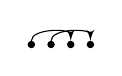
\begin{tikzpicture}[yscale=0.08,xscale=0.09,inner sep=.8pt,node distance=.25cm,>=latex']%,>=stealth',->]
\draw node [draw,circle,fill=black] (U1)               {};
\draw node [draw,circle,fill=black] [right of=U1] (U2) {};
\draw node [draw,circle,fill=black] [right of=U2] (U3) {};
\draw node [draw,circle,fill=black] [right of=U3] (U4) {};
\draw [->] (U1.north) .. controls ($ (U1.north) + (0,2) $) and ($ (U3.north) + (0,2) $) .. (U3.north);
\draw [->] (U2.north) .. controls ($ (U2.north) + (0,2) $) and ($ (U4.north) + (0,2) $) .. (U4.north);
\end{tikzpicture}
}% end \CrossingLL

\newcommand{\LabeledCrossingLR}[5]{%
\begin{tikzpicture}[scale=#1,inner sep=.8pt,node distance=.45cm,>=latex',
                    text height=1.5ex,text depth=.25ex]
\draw node [] (U1)               {#2};
\draw node [] [right of=U1] (U2) {#3};
\draw node [] [right of=U2] (U3) {#4};
\draw node [] [right of=U3] (U4) {#5};
\draw [->] (U1.north) .. controls ($ (U1.north) + (0,1.5) $) and ($ (U3.north) + (0,1.5) $) .. (U3.north);
\draw [<-] (U2.north) .. controls ($ (U2.north) + (0,1.5) $) and ($ (U4.north) + (0,1.5) $) .. (U4.north);
\end{tikzpicture}
}% end \LabeledCrossingLR

\newcommand{\CrossingLR}{%
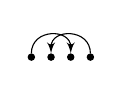
\begin{tikzpicture}[yscale=0.08,xscale=0.09,inner sep=.8pt,node distance=.25cm,>=latex']%,>=stealth',->]
\draw node [draw,circle,fill=black] (U1)               {};
\draw node [draw,circle,fill=black] [right of=U1] (U2) {};
\draw node [draw,circle,fill=black] [right of=U2] (U3) {};
\draw node [draw,circle,fill=black] [right of=U3] (U4) {};
\draw [->] (U1.north) .. controls ($ (U1.north) + (0,4) $) and ($ (U3.north) + (0,4) $) .. (U3.north);
\draw [<-] (U2.north) .. controls ($ (U2.north) + (0,4) $) and ($ (U4.north) + (0,4) $) .. (U4.north);
\end{tikzpicture}
}% end \CrossingLR

\newcommand{\LabeledCrossingRL}[5]{%
\begin{tikzpicture}[scale=#1,inner sep=.8pt,node distance=.45cm,>=latex',
                    text height=1.5ex,text depth=.25ex]
\draw node [] (U1)               {#2};
\draw node [] [right of=U1] (U2) {#3};
\draw node [] [right of=U2] (U3) {#4};
\draw node [] [right of=U3] (U4) {#5};
\draw [<-] (U1.north) .. controls ($ (U1.north) + (0,1.5) $) and ($ (U3.north) + (0,1.5) $) .. (U3.north);
\draw [->] (U2.north) .. controls ($ (U2.north) + (0,1.5) $) and ($ (U4.north) + (0,1.5) $) .. (U4.north);
\end{tikzpicture}
}% end \LabeledCrossingRL

\newcommand{\CrossingRL}{%
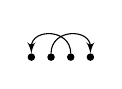
\begin{tikzpicture}[yscale=0.08,xscale=0.09,inner sep=.8pt,node distance=.25cm,>=latex']%,>=stealth',->]
\draw node [draw,circle,fill=black] (U1)               {};
\draw node [draw,circle,fill=black] [right of=U1] (U2) {};
\draw node [draw,circle,fill=black] [right of=U2] (U3) {};
\draw node [draw,circle,fill=black] [right of=U3] (U4) {};
\draw [<-] (U1.north) .. controls ($ (U1.north) + (0,4) $) and ($ (U3.north) + (0,4) $) .. (U3.north);
\draw [->] (U2.north) .. controls ($ (U2.north) + (0,4) $) and ($ (U4.north) + (0,4) $) .. (U4.north);
\end{tikzpicture}
}% end \CrossingRL

\newcommand{\LabeledCrossingRR}[5]{%
\begin{tikzpicture}[scale=#1,inner sep=.8pt,node distance=.45cm,>=latex',
                    text height=1.5ex,text depth=.25ex]
\draw node [] (U1)               {#2};
\draw node [] [right of=U1] (U2) {#3};
\draw node [] [right of=U2] (U3) {#4};
\draw node [] [right of=U3] (U4) {#5};
\draw [<-] (U1.north) .. controls ($ (U1.north) + (0,1.5) $) and ($ (U3.north) + (0,1.5) $) .. (U3.north);
\draw [<-] (U2.north) .. controls ($ (U2.north) + (0,1.5) $) and ($ (U4.north) + (0,1.5) $) .. (U4.north);
\end{tikzpicture}
}% end \LabeledCrossingRR

\newcommand{\CrossingRR}{%
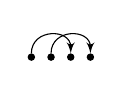
\begin{tikzpicture}[yscale=0.08,xscale=0.09,inner sep=.8pt,node distance=.25cm,>=latex']%,>=stealth',->]
\draw node [draw,circle,fill=black] (U1)               {};
\draw node [draw,circle,fill=black] [right of=U1] (U2) {};
\draw node [draw,circle,fill=black] [right of=U2] (U3) {};
\draw node [draw,circle,fill=black] [right of=U3] (U4) {};
\draw [->] (U1.north) .. controls ($ (U1.north) + (0,4) $) and ($ (U3.north) + (0,4) $) .. (U3.north);
\draw [->] (U2.north) .. controls ($ (U2.north) + (0,4) $) and ($ (U4.north) + (0,4) $) .. (U4.north);
\end{tikzpicture}
}% end \CrossingRR

\newcommand{\Inclusion}{%
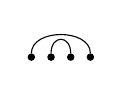
\begin{tikzpicture}[yscale=0.08,xscale=0.09,inner sep=.8pt,node distance=.25cm,>=latex']
\draw node [draw,circle,fill=black] (U1)               {};
\draw node [draw,circle,fill=black] [right of=U1] (U2) {};
\draw node [draw,circle,fill=black] [right of=U2] (U3) {};
\draw node [draw,circle,fill=black] [right of=U3] (U4) {};
\draw [] (U1.north) .. controls ($ (U1.north) + (0,4) $) and ($ (U4.north) + (0,4) $) .. (U4.north);
\draw [] (U2.north) .. controls ($ (U2.north) + (0,3) $) and ($ (U3.north) + (0,3) $) .. (U3.north);
\end{tikzpicture}
}% end \Inclusion

\newcommand{\LabeledInclusionLL}[5]{%
\begin{tikzpicture}[scale=#1,inner sep=.8pt,node distance=.45cm,>=latex',
                    text height=1.5ex,text depth=.25ex]
\draw node [] (U1)               {#2};
\draw node [] [right of=U1] (U2) {#3};
\draw node [] [right of=U2] (U3) {#4};
\draw node [] [right of=U3] (U4) {#5};
\draw [->] (U1.north) .. controls ($ (U1.north) + (0,2) $) and ($ (U4.north) + (0,2) $) .. (U4.north);
\draw [->] (U2.north) .. controls ($ (U2.north) + (0,1) $) and ($ (U3.north) + (0,1) $) .. (U3.north);
\end{tikzpicture}
}% end \LabeledInclusionLL

\newcommand{\InclusionLL}{%
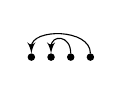
\begin{tikzpicture}[yscale=0.08,xscale=0.09,inner sep=.8pt,node distance=.25cm,>=latex']
\draw node [draw,circle,fill=black] (U1)               {};
\draw node [draw,circle,fill=black] [right of=U1] (U2) {};
\draw node [draw,circle,fill=black] [right of=U2] (U3) {};
\draw node [draw,circle,fill=black] [right of=U3] (U4) {};
+\draw [->] (U4.north) .. controls ($ (U4.north) + (0,4) $) and ($ (U1.north) + (0,4) $) .. (U1.north);
+\draw [->] (U3.north) .. controls ($ (U3.north) + (0,3) $) and ($ (U2.north) + (0,3) $) .. (U2.north);
\end{tikzpicture}
}% end \InclusionLL

\newcommand{\LabeledInclusionLR}[5]{%
\begin{tikzpicture}[scale=#1,inner sep=.8pt,node distance=.45cm,>=latex',
                    text height=1.5ex,text depth=.25ex]
\draw node [] (U1)               {#2};
\draw node [] [right of=U1] (U2) {#3};
\draw node [] [right of=U2] (U3) {#4};
\draw node [] [right of=U3] (U4) {#5};
\draw [->] (U1.north) .. controls ($ (U1.north) + (0,2) $) and ($ (U4.north) + (0,2) $) .. (U4.north);
\draw [<-] (U2.north) .. controls ($ (U2.north) + (0,1) $) and ($ (U3.north) + (0,1) $) .. (U3.north);
\end{tikzpicture}
}% end \LabeledInclusionLR

\newcommand{\InclusionLR}{%
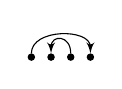
\begin{tikzpicture}[yscale=0.08,xscale=0.09,inner sep=.8pt,node distance=.25cm,>=latex']
\draw node [draw,circle,fill=black] (U1)               {};
\draw node [draw,circle,fill=black] [right of=U1] (U2) {};
\draw node [draw,circle,fill=black] [right of=U2] (U3) {};
\draw node [draw,circle,fill=black] [right of=U3] (U4) {};
\draw [->] (U1.north) .. controls ($ (U1.north) + (0,4) $) and ($ (U4.north) + (0,4) $) .. (U4.north);
\draw [<-] (U2.north) .. controls ($ (U2.north) + (0,3) $) and ($ (U3.north) + (0,3) $) .. (U3.north);
\end{tikzpicture}
}% end \InclusionLR

\newcommand{\LabeledInclusionRL}[5]{%
\begin{tikzpicture}[scale=#1,inner sep=.8pt,node distance=.45cm,>=latex',
                    text height=1.5ex,text depth=.25ex]
\draw node [] (U1)               {#2};
\draw node [] [right of=U1] (U2) {#3};
\draw node [] [right of=U2] (U3) {#4};
\draw node [] [right of=U3] (U4) {#5};
\draw [<-] (U1.north) .. controls ($ (U1.north) + (0,2) $) and ($ (U4.north) + (0,2) $) .. (U4.north);
\draw [->] (U2.north) .. controls ($ (U2.north) + (0,1) $) and ($ (U3.north) + (0,1) $) .. (U3.north);
\end{tikzpicture}
}% end \LabeledInclusionRL

\newcommand{\InclusionRL}{%
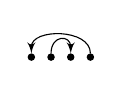
\begin{tikzpicture}[yscale=0.08,xscale=0.09,inner sep=.8pt,node distance=.25cm,>=latex']
\draw node [draw,circle,fill=black] (U1)               {};
\draw node [draw,circle,fill=black] [right of=U1] (U2) {};
\draw node [draw,circle,fill=black] [right of=U2] (U3) {};
\draw node [draw,circle,fill=black] [right of=U3] (U4) {};
\draw [<-] (U1.north) .. controls ($ (U1.north) + (0,4) $) and ($ (U4.north) + (0,4) $) .. (U4.north);
\draw [->] (U2.north) .. controls ($ (U2.north) + (0,3) $) and ($ (U3.north) + (0,3) $) .. (U3.north);
\end{tikzpicture}
}% end \InclusionRL

\newcommand{\LabeledInclusionRR}[5]{%
\begin{tikzpicture}[scale=#1,inner sep=.8pt,node distance=.45cm,>=latex',
                    text height=1.5ex,text depth=.25ex]
\draw node [] (U1)               {#2};
\draw node [] [right of=U1] (U2) {#3};
\draw node [] [right of=U2] (U3) {#4};
\draw node [] [right of=U3] (U4) {#5};
\draw [<-] (U1.north) .. controls ($ (U1.north) + (0,2) $) and ($ (U4.north) + (0,2) $) .. (U4.north);
\draw [<-] (U2.north) .. controls ($ (U2.north) + (0,1) $) and ($ (U3.north) + (0,1) $) .. (U3.north);
\end{tikzpicture}
}% end \LabeledInclusionRR

\newcommand{\InclusionRR}{%
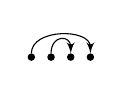
\begin{tikzpicture}[yscale=0.08,xscale=0.09,inner sep=.8pt,node distance=.25cm,>=latex']
\draw node [draw,circle,fill=black] (U1)               {};
\draw node [draw,circle,fill=black] [right of=U1] (U2) {};
\draw node [draw,circle,fill=black] [right of=U2] (U3) {};
\draw node [draw,circle,fill=black] [right of=U3] (U4) {};
\draw [->] (U1.north) .. controls ($ (U1.north) + (0,4) $) and ($ (U4.north) + (0,4) $) .. (U4.north);
\draw [->] (U2.north) .. controls ($ (U2.north) + (0,3) $) and ($ (U3.north) + (0,3) $) .. (U3.north);
\end{tikzpicture}
}% end \InclusionRR

\newcommand{\Precedence}{%

\begin{tikzpicture}[yscale=0.08,xscale=0.09,inner sep=.8pt,node distance=.25cm,>=latex']
\draw node [draw,circle,fill=black] (U1)               {};
\draw node [draw,circle,fill=black] [right of=U1] (U2) {};
\draw node [draw,circle,fill=black] [right of=U2] (U3) {};
\draw node [draw,circle,fill=black] [right of=U3] (U4) {};
\draw [] (U1.north) .. controls ($ (U1.north) + (0,4) $) and ($ (U2.north) + (0,4) $) .. (U2.north);
\draw [] (U3.north) .. controls ($ (U3.north) + (0,4) $) and ($ (U4.north) + (0,4) $) .. (U4.north);
\end{tikzpicture}
}% end \Precedence

\newcommand{\LabeledPrecedenceLL}[5]{%
\begin{tikzpicture}[scale=#1,inner sep=.8pt,node distance=.45cm,>=latex',
                    text height=1.5ex,text depth=.25ex]
\draw node [] (U1)               {#2};
\draw node [] [right of=U1] (U2) {#3};
\draw node [] [right of=U2] (U3) {#4};
\draw node [] [right of=U3] (U4) {#5};
\draw [->] (U1.north) .. controls ($ (U1.north) + (0,1.5) $) and ($ (U2.north) + (0,1.5) $) .. (U2.north);
\draw [->] (U3.north) .. controls ($ (U3.north) + (0,1.5) $) and ($ (U4.north) + (0,1.5) $) .. (U4.north);
\end{tikzpicture}
}% end \PrecedenceLL

\newcommand{\PrecedenceLL}{%
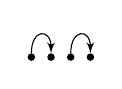
\begin{tikzpicture}[yscale=0.08,xscale=0.09,inner sep=.8pt,node distance=.25cm,>=latex']
\draw node [draw,circle,fill=black] (U1)               {};
\draw node [draw,circle,fill=black] [right of=U1] (U2) {};
\draw node [draw,circle,fill=black] [right of=U2] (U3) {};
\draw node [draw,circle,fill=black] [right of=U3] (U4) {};
\draw [->] (U1.north) .. controls ($ (U1.north) + (0,4) $) and ($ (U2.north) + (0,4) $) .. (U2.north);
\draw [->] (U3.north) .. controls ($ (U3.north) + (0,4) $) and ($ (U4.north) + (0,4) $) .. (U4.north);
\end{tikzpicture}
}% end \PrecedenceLL

\newcommand{\LabeledPrecedenceLR}[5]{%
\begin{tikzpicture}[scale=#1,inner sep=.8pt,node distance=.45cm,>=latex',
                    text height=1.5ex,text depth=.25ex]
\draw node [] (U1)               {#2};
\draw node [] [right of=U1] (U2) {#3};
\draw node [] [right of=U2] (U3) {#4};
\draw node [] [right of=U3] (U4) {#5};
\draw [->] (U1.north) .. controls ($ (U1.north) + (0,1.5) $) and ($ (U2.north) + (0,1.5) $) .. (U2.north);
\draw [<-] (U3.north) .. controls ($ (U3.north) + (0,1.5) $) and ($ (U4.north) + (0,1.5) $) .. (U4.north);
\end{tikzpicture}
}% end \PrecedenceLR

\newcommand{\PrecedenceLR}{%
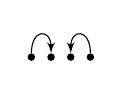
\begin{tikzpicture}[yscale=0.08,xscale=0.09,inner sep=.8pt,node distance=.25cm,>=latex']
\draw node [draw,circle,fill=black] (U1)               {};
\draw node [draw,circle,fill=black] [right of=U1] (U2) {};
\draw node [draw,circle,fill=black] [right of=U2] (U3) {};
\draw node [draw,circle,fill=black] [right of=U3] (U4) {};
\draw [->] (U1.north) .. controls ($ (U1.north) + (0,4) $) and ($ (U2.north) + (0,4) $) .. (U2.north);
\draw [<-] (U3.north) .. controls ($ (U3.north) + (0,4) $) and ($ (U4.north) + (0,4) $) .. (U4.north);
\end{tikzpicture}
}% end \PrecedenceLR

\newcommand{\LabeledPrecedenceRL}[5]{%
\begin{tikzpicture}[scale=#1,inner sep=.8pt,node distance=.45cm,>=latex',
                    text height=1.5ex,text depth=.25ex]
\draw node [] (U1)               {#2};
\draw node [] [right of=U1] (U2) {#3};
\draw node [] [right of=U2] (U3) {#4};
\draw node [] [right of=U3] (U4) {#5};
\draw [<-] (U1.north) .. controls ($ (U1.north) + (0,1.5) $) and ($ (U2.north) + (0,1.5) $) .. (U2.north);
\draw [->] (U3.north) .. controls ($ (U3.north) + (0,1.5) $) and ($ (U4.north) + (0,1.5) $) .. (U4.north);
\end{tikzpicture}
}% end \PrecedenceRL

\newcommand{\PrecedenceRL}{%
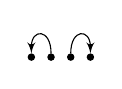
\begin{tikzpicture}[yscale=0.08,xscale=0.09,inner sep=.8pt,node distance=.25cm,>=latex']
\draw node [draw,circle,fill=black] (U1)               {};
\draw node [draw,circle,fill=black] [right of=U1] (U2) {};
\draw node [draw,circle,fill=black] [right of=U2] (U3) {};
\draw node [draw,circle,fill=black] [right of=U3] (U4) {};
\draw [<-] (U1.north) .. controls ($ (U1.north) + (0,4) $) and ($ (U2.north) + (0,4) $) .. (U2.north);
\draw [->] (U3.north) .. controls ($ (U3.north) + (0,4) $) and ($ (U4.north) + (0,4) $) .. (U4.north);
\end{tikzpicture}
}% end \PrecedenceRL

\newcommand{\LabeledPrecedenceRR}[5]{%
\begin{tikzpicture}[scale=#1,inner sep=.8pt,node distance=.45cm,>=latex',
                    text height=1.5ex,text depth=.25ex]
\draw node [] (U1)               {#2};
\draw node [] [right of=U1] (U2) {#3};
\draw node [] [right of=U2] (U3) {#4};
\draw node [] [right of=U3] (U4) {#5};
\draw [<-] (U1.north) .. controls ($ (U1.north) + (0,1.5) $) and ($ (U2.north) + (0,1.5) $) .. (U2.north);
\draw [<-] (U3.north) .. controls ($ (U3.north) + (0,1.5) $) and ($ (U4.north) + (0,1.5) $) .. (U4.north);
\end{tikzpicture}
}% end \PrecedenceRR

\newcommand{\PrecedenceRR}{%
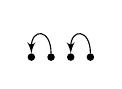
\begin{tikzpicture}[yscale=0.08,xscale=0.09,inner sep=.8pt,node distance=.25cm,>=latex']
\draw node [draw,circle,fill=black] (U1)               {};
\draw node [draw,circle,fill=black] [right of=U1] (U2) {};
\draw node [draw,circle,fill=black] [right of=U2] (U3) {};
\draw node [draw,circle,fill=black] [right of=U3] (U4) {};
\draw [<-] (U1.north) .. controls ($ (U1.north) + (0,4) $) and ($ (U2.north) + (0,4) $) .. (U2.north);
\draw [<-] (U3.north) .. controls ($ (U3.north) + (0,4) $) and ($ (U4.north) + (0,4) $) .. (U4.north);
\end{tikzpicture}
}% end \PrecedenceRR

%%%%%%%%%%%%%%%%%%%%%%%%%%%%%%%%%%%%%%%%%%%%%%%%%%%%%%%%%%%%%%%%%%%%%%%%%%%%%%

%%% 
%%% complexity.tex
%%% 

\usepackage{xspace}

%%% ----------------------------------------------------------------------
%%% complexity classes
%%% ----------------------------------------------------------------------

% TIME
\newcommand{\DTIMEX}{{\sf\bf DTIME}}
\newcommand{\DTIMEclass}{\DTIMEX\xspace}
\newcommand{\DTIME}{\DTIMEclass}
% NL class
\newcommand{\NLclassbase}{{\sf\bf NL}}
\newcommand{\NLclass}{\NLclassbase\xspace}
% P class
\newcommand{\Pclassbase}{{\sf\bf P}}
\newcommand{\Pclass}{\Pclassbase\xspace}
% NP class
\newcommand{\NPclassbase}{{\sf\bf NP}}
\newcommand{\NPclass}{\NPclassbase\xspace}
% coNP class
\newcommand{\coNPclassbase}{{\sf\bf coNP}}
\newcommand{\coNPclass}{\coNPclassbase\xspace}
% PSPACE class
\newcommand{\PSPACEclassbase}{{\sf\bf PSPACE}}
\newcommand{\PSPACEclass}{\PSPACEclassbase\xspace}
% MAXSNP class
\newcommand{\MaxSNPclassbase}{{\sf\bf MaxSNP}}
\newcommand{\MaxSNPclass}{\MaxSNPclassbase\xspace}
% MAXNP class
\newcommand{\MaxNPclassbase}{{\sf\bf MaxNP}}
\newcommand{\MaxNPclass}{\MaxNPclassbase\xspace}
% EPTAS class
\newcommand{\EPTASclassbase}{{\sf\bf EPTAS}}
\newcommand{\EPTASclass}{\EPTASclassbase\xspace}
% FPTAS class
\newcommand{\FPTASclassbase}{{\sf\bf FPTAS}}
\newcommand{\FPTASclass}{\FPTASclassbase\xspace}
% PTAS class
\newcommand{\PTASclassbase}{{\sf\bf PTAS}}
\newcommand{\PTASclass}{\PTASclassbase\xspace}
% APX class
\newcommand{\APXclassbase}{{\sf\bf APX}}
\newcommand{\APXclass}{\APXclassbase\xspace}
% log-APX class
\newcommand{\logAPXclassbase}{{\sf\bf log{\tt -}APX}}
\newcommand{\logAPXclass}{\logAPXclassbase\xspace}
% poly-APX class
\newcommand{\polyAPXclassbase}{{\sf\bf poly{\tt -}APX}}
\newcommand{\polyAPXclass}{\polyAPXclassbase\xspace}
% exp-APX class
\newcommand{\expAPXclassbase}{{\sf\bf exp{\tt -}APX}}
\newcommand{\expAPXclass}{\expAPXclassbase\xspace}
% NPO class
\newcommand{\NPOclassbase}{{\sf\bf NPO}}
\newcommand{\NPOclass}{\NPOclassbase\xspace}
% #P class
\newcommand{\sharpPclassbase}{\#{\sf\bf P}}
\newcommand{\sharpPclass}{\sharpPclassbase\xspace}
% FPT class
\newcommand{\FPTclassbase}{{\sf\bf FPT}}
\newcommand{\FPTclass}{\FPTclassbase\xspace}
% W class
\newcommand{\Wclassbase}[1]{{\sf\bf W[#1]}}
\newcommand{\Wclass}[1]{\Wclassbase{#1}\xspace}
% W class
\newcommand{\XPclassbase}{{\sf\bf XP}}
\newcommand{\XPclass}{\XPclassbase\xspace}
% WNL class
\newcommand{\WNLclassbase}{{\sf\bf WNL}}
\newcommand{\WNLclass}{\WNLclassbase\xspace}
% ZPP class
\newcommand{\ZPPclassbase}{{\sf\bf ZPP}}
\newcommand{\ZPPclass}{\ZPPclassbase\xspace}
% NPK class
\newcommand{\NPKclassbase}{{\sf\bf NPK}}
\newcommand{\NPKclass}{\NPKclassbase\xspace}
\newcommand{\NPKandclass}{\text{$\NPKclass_\text{and}$}\xspace}
\newcommand{\NPKzeroandclass}{\text{$\NPKclass^0_\text{and}$}\xspace}
\newcommand{\NPKorclass}{\text{$\NPKclass_\text{or}$}\xspace}
\newcommand{\NPKzeroorclass}{\text{$\NPKclass^0_\text{or}$}\xspace}

%%% ----------------------------------------------------------------------
%%% complete
%%% ----------------------------------------------------------------------

% keyword
\newcommand{\complete}{\text{-complete}}
% NL-complete
\newcommand{\NLcomplete}{\NLclassbase\complete\xspace}
\newcommand{\NLC}{\NLcomplete}
% P-complete
\newcommand{\Pcomplete}{\Pclassbase\complete\xspace}
\newcommand{\PC}{\Pcomplete}
% NP-complete
\newcommand{\NPcomplete}{\NPclassbase\complete\xspace}
\newcommand{\NPC}{\NPcomplete}
% coNP-complete
\newcommand{\coNPcomplete}{\coNPclassbase\complete\xspace}
\newcommand{\coNPC}{\coNPcomplete}
% PSPACE-complete
\newcommand{\PSPACEcomplete}{\PSPACEclassbase\complete\xspace}
\newcommand{\PSPACEC}{\PSPACEcomplete}
% MAXSNP-complete
\newcommand{\MaxSNPcomplete}{\MaxSNPclassbase\complete\xspace}
\newcommand{\MaxSNPC}{\MaxSNPcomplete}
% APX-complete
\newcommand{\APXcomplete}{\APXclassbase\complete\xspace}
\newcommand{\APXC}{\APXcomplete}
% #P-complete
\newcommand{\sharpPcomplete}{\sharpPclassbase\complete\xspace}
\newcommand{\sharpPC}{\sharpPcomplete}
% W[i]-complete
\newcommand{\Wcomplete}[1]{\Wclassbase{#1}\complete\xspace}
\newcommand{\WC}[1]{\Wcomplete{#1}}
% WNL-complete
\newcommand{\WNLcomplete}{\WNLclassbase\complete\xspace}
\newcommand{\WNLC}{\WNLcomplete}

%%% ----------------------------------------------------------------------
%%% hard
%%% ----------------------------------------------------------------------

% keyword
\newcommand{\hard}{\text{-hard}}
% NL-hard
\newcommand{\NLhard}{\NLclassbase\hard\xspace}
\newcommand{\NLH}{\NLhard}
% P-hard
\newcommand{\Phard}{\NPclassbase\hard\xspace}
\newcommand{\PH}{\Phard}
% NP-hard
\newcommand{\NPhard}{\NPclassbase\hard\xspace}
\newcommand{\NPH}{\NPhard}
% coNP-hard
\newcommand{\coNPhard}{\coNPclassbase\hard\xspace}
\newcommand{\coNPH}{\coNPhard}
% PSPACE-hard
\newcommand{\PSPACEhard}{\PSPACEclassbase\hard\xspace}
\newcommand{\PSPACEH}{\PSPACEhard}
% MAXSNP-hard
\newcommand{\MaxSNPhard}{\MaxSNPclassbase\hard\xspace}
\newcommand{\MaxSNPH}{\MaxSNPhard}
% APX-hard
\newcommand{\APXhard}{\APXclassbase\hard\xspace}
\newcommand{\APXH}{\APXhard}
% WNL-hard
\newcommand{\WNLhard}{\WNLclassbase\hard\xspace}
\newcommand{\WNLH}{\WNLhard}
% #P-hard
\newcommand{\sharpPhard}{\sharpPclassbase\hard\xspace}
\newcommand{\sharpPH}{\sharpPhard}
% W[i]-hard
\newcommand{\Whard}[1]{\Wclassbase{#1}\hard\xspace}
\newcommand{\WH}[1]{\Whard{#1}}

%%% ----------------------------------------------------------------------
%%% hardness
%%% ----------------------------------------------------------------------

% keyword
\newcommand{\hardness}{\text{-hardness}}
% NP-hardness
\newcommand{\NPhardness}{\NPclassbase\hardness\xspace}
% APX-hardness
\newcommand{\APXhardness}{\APXclassbase\hardness\xspace}
% W[i]-hardness
\newcommand{\Whardness}[1]{\Wclassbase{#1}\hardness\xspace}
% WNL-hardness
\newcommand{\WNLhardness}{\WNLclassbase\hardness\xspace}

%%% ----------------------------------------------------------------------
%%% completeness
%%% ----------------------------------------------------------------------

% keyword
\newcommand{\completeness}{\text{-completeness}}
% NL-completeness
\newcommand{\NLcompleteness}{\NLclassbase\completeness\xspace}
% P-completeness
\newcommand{\Pcompleteness}{\NPclassbase\completeness\xspace}
% NP-completeness
\newcommand{\NPcompleteness}{\NPclassbase\completeness\xspace}
% APX-completeness
\newcommand{\APXcompleteness}{\APXclassbase\completeness\xspace}
% #P-completeness
\newcommand{\sharpPcompleteness}{\sharpPclassbase\completeness\xspace}
% W[i]-hard
\newcommand{\Wcompleteness}[1]{\W{#1}-\completeness\xspace}

%%% ----------------------------------------------------------------------
%%% reduction
%%% ----------------------------------------------------------------------

\newcommand{\reduction}{reduction}
\newcommand{\reductions}{reductions}
\newcommand{\reductible}{reductible}

\newcommand{\APTypeReduction}{AP}
\newcommand{\PTASTypeReduction}{PTAS}
\newcommand{\LTypeReduction}{L}
\newcommand{\ETypeReduction}{E}
\newcommand{\fptTypeReduction}{fpt}
\newcommand{\pptTypeReduction}{ptp}

% AP-reduction
\newcommand{\APreduction}{\APTypeReduction-\reduction\xspace}
\newcommand{\APreductions}{\APTypeReduction-\reductions\xspace}
\newcommand{\APreductible}{\APTypeReduction-\reductible\xspace}

% PTAS-reduction
\newcommand{\PTASeduction}{\PTASTypeReduction-\reduction\xspace}
\newcommand{\PTASreductions}{\PTASTypeReduction-\reductions\xspace}
\newcommand{\PTASreductible}{\PTASTypeReduction-\reductible\xspace}

% L-reduction
\newcommand{\Lreduction}{\LTypeReduction-\reduction\xspace}
\newcommand{\Lreductions}{\LTypeReduction-\reductions\xspace}
\newcommand{\Lreductible}{\LTypeReduction-\reductible\xspace}

% E-reduction
\newcommand{\Ereduction}{\ETypeReduction-\reduction\xspace}
\newcommand{\Ereductions}{\ETypeReduction-\reductions\xspace}
\newcommand{\Ereductible}{\ETypeReduction-\reductible\xspace}

% fpt-reduction
\newcommand{\fptreduction}{\fptTypeReduction-\reduction\xspace}
\newcommand{\fptreductions}{\fptTypeReduction-\reductions\xspace}
\newcommand{\fptreductible}{\fptTypeReduction-\reductible\xspace}

% ptp-reduction
\newcommand{\ptpreduction}{\ptpTypeReduction-\reduction\xspace}
\newcommand{\ptpreductions}{\ptpTypeReduction-\reductions\xspace}
\newcommand{\ptpreductible}{\ptpTypeReduction-\reductible\xspace}

% symbols
\DeclareMathOperator{\APreduce}{\text{$\leq_{\text{\APTypeReduction}}$}}
\DeclareMathOperator{\PTASreduce}{\text{$\leq_{\text{\PTASTypeReduction}}$}}
\DeclareMathOperator{\Lreduce}{\text{$\leq_{\text{\LTypeReduction}}$}}
\DeclareMathOperator{\Ereduce}{\text{$\leq_{\text{\ETypeReduction}}$}}
\DeclareMathOperator{\fptreduce}{\text{$\leq_{\text{\fptTypeReduction}}$}}
\DeclareMathOperator{\ptpreduce}{\text{$\leq_{\text{\fptTypeReduction}}$}}

%% 
%% Approximation
%%
\DeclareMathOperator{\poly}{poly}
\DeclareMathOperator{\POLY}{poly}
\DeclareMathOperator{\SIZE}{size}
\newcommand{\sol}{{\sf sol}\xspace}
\newcommand{\PB}[1]{\textsf{\scshape{#1}}}
\newcommand{\OPTname}{opt}
\newcommand{\OPT}{\text{$\mathsf{\bf \OPTname}$}}
\newcommand{\OPTpb}[1]{\text{$\mathsf{\OPTname}_{\PB{#1}}$}}
\newcommand{\ALGO}[1]{\textbf{\ttfamily\sf #1}}
\newcommand{\Approxname}{Approx}
\newcommand{\APPROX}[1]{\text{$\ALGO{\Approxname}_{\,\PB{#1}}$}}
\newcommand{\PCP}{{\sf\bf PCP}\xspace}

%%
%% Problem Definition
%%
\newcommand{\PbDef}[3]{%
\begin{center}
  \begin{tabular}{l}%
    \shadowbox{%
    \begin{minipage}[c]{.9\textwidth}
      \smallskip%
      \par\noindent%
      {#1}%
      \smallskip
      \par\noindent%
      $\bullet$
      \textbf{\textsf{Input}}~: #2% 
      \medskip
      \par\noindent%
      $\bullet$
      \textbf{\textsf{Question}}~:
      #3% 
      \smallskip%
      \par\noindent%
    \end{minipage}
  }% end shadowbox
  \end{tabular}%
\end{center}
}%
\newcommand{\PbDefinition}{\PbDef}

%%
%% Problem (Input + Output) Definition
%%
\newcommand{\PbInputOutputDef}[3]{%
\begin{center}
  \begin{tabular}{l}%
    \shadowbox{%
    \begin{minipage}[c]{.9\textwidth}
      \smallskip%
      \par\noindent%
      \PB{#1}%
      \medskip%
      \par\noindent%
      $\bullet$
      \textbf{\textsf{Input}}~: #2% 
      \medskip
      \par\noindent%
      $\bullet$
      \textbf{\textsf{Output}}~:
      #3% 
      \smallskip%
      \par\noindent%
    \end{minipage}
  }% end shadowbox
  \end{tabular}%
\end{center}
}%
\newcommand{\PbInputOutputDefinition}{\PbInputOutputDef}


%%
%% Optimization Problem Definition
%%

\newcommand{\OptPbDefinition}[4]{%
\begin{center}
  \begin{tabular}{l}%
    \shadowbox{%
    \begin{minipage}[c]{.9\textwidth}
      \par\noindent%
      \shadowbox{#1}%
      \par\noindent%
      $\bullet$
      \textbf{\textsf{Input}}~: #2% 
      \par\noindent%
      $\bullet$
      \textbf{\textsf{Solution}}~: #3%  
      \par\noindent%
      $\bullet$
      \textbf{\textsf{Measure}}~: #4% 
      \par\noindent%
    \end{minipage}
    }% end shadowbox
  \end{tabular}%
\end{center}
}%

%%
%% Parameterized Problem Definition
%%
\newcommand{\ParamPbDefinition}[4]{%
\begin{center}
  \begin{tabular}{l}%
    %\shadowbox{%
    \begin{minipage}[c]{.95\textwidth}
      % \smallskip%
      \par\noindent%
      #1%
      % \smallskip%
      \par\noindent%
      \textbf{\textsf{Input}}~: #2% 
      % \smallskip
      \par\noindent%
      \textbf{\textsf{Question}}~: #3%  
      % \smallskip
      \par\noindent%
      \textbf{\textsf{Parameter}}~: #4% 
      %\smallskip%
      \par\noindent%
    \end{minipage}
  %}% end shadowbox
  \end{tabular}%
\end{center}
}%
\newcommand{\ParamPbDefinitionTwo}[5]{%
\begin{center}
  \begin{tabular}{l}%
    \shadowbox{%
    \begin{minipage}[c]{.9\textwidth}
      \smallskip%
      \par\noindent%
      \shadowbox{#1}%
      \medskip%
      \par\noindent%
      $\bullet$
      \textbf{\textsf{Input}}~: #2% 
%      \medskip
      \par\noindent%
      $\bullet$
      \textbf{\textsf{Parameter}}~: #3% 
 %     \medskip
      \par\noindent%
      $\bullet$
      \textbf{\textsf{Parameter}}~: #4% 
      \medskip
      \par\noindent%
      $\bullet$
      \textbf{\textsf{Question}}~: #5%  
      \smallskip%
      \par\noindent%
    \end{minipage}
    }% end shadowbox
  \end{tabular}%
\end{center}
}%
\newcommand{\ParamPbDefinitionThree}[6]{%
\begin{center}
  \begin{tabular}{l}%
    \shadowbox{%
    \begin{minipage}[c]{.9\textwidth}
      \smallskip%
      \par\noindent%
      \shadowbox{#1}%
      \medskip%
      \par\noindent%
      $\bullet$
      \textbf{\textsf{Input}}~: #2% 
%      \medskip
      \par\noindent%
      $\bullet$
      \textbf{\textsf{Parameter}}~: #3% 
%      \medskip
      \par\noindent%
      $\bullet$
      \textbf{\textsf{Parameter}}~: #4% 
%      \medskip
      \par\noindent%
      $\bullet$
      \textbf{\textsf{Parameter}}~: #5%  
      \medskip
      \par\noindent%
      $\bullet$
      \textbf{\textsf{Question}}~: #6%  
      \smallskip%
      \par\noindent%
    \end{minipage}
    }% end shadowbox
  \end{tabular}%
\end{center}
}%
\newcommand{\ParamPbDefinitionFour}[7]{%
\begin{center}
  \begin{tabular}{l}%
    \shadowbox{%
    \begin{minipage}[c]{.9\textwidth}
      \smallskip%
      \par\noindent%
      \shadowbox{#1}%
      \medskip%
      \par\noindent%
      $\bullet$
      \textbf{\textsf{Input}}~: #2% 
%      \medskip
      \par\noindent%
      $\bullet$
      \textbf{\textsf{Parameter}}~: #3% 
%      \medskip
      \par\noindent%
      $\bullet$
      \textbf{\textsf{Parameter}}~: #4% 
%      \medskip
      \par\noindent%
      $\bullet$
      \textbf{\textsf{Parameter}}~: #5%  
%      \medskip
      \par\noindent%
    $\bullet$
      \textbf{\textsf{Parameter}}~: #6%  
      \medskip
      \par\noindent%
      $\bullet$
      \textbf{\textsf{Question}}~: #7%  
      \smallskip%
      \par\noindent%
    \end{minipage}
    }% end shadowbox
  \end{tabular}%
\end{center}
}%
\newcommand{\ParamPbDefinitionFive}[8]{%
\begin{center}
  \begin{tabular}{l}%
    \shadowbox{%
    \begin{minipage}[c]{.9\textwidth}
      \smallskip%
      \par\noindent%
      \shadowbox{#1}%
      \medskip%
      \par\noindent%
      $\bullet$
      \textbf{\textsf{Input}}~: #2% 
%      \medskip
      \par\noindent%
      $\bullet$
      \textbf{\textsf{Parameter}}~: #3% 
%      \medskip
      \par\noindent%
      $\bullet$
      \textbf{\textsf{Parameter}}~: #4% 
%      \medskip
      \par\noindent%
      $\bullet$
      \textbf{\textsf{Parameter}}~: #5%  
%      \medskip
      \par\noindent%
    $\bullet$
      \textbf{\textsf{Parameter}}~: #6%  
%      \medskip
      \par\noindent%
    $\bullet$
      \textbf{\textsf{Parameter}}~: #7%  
      \medskip
      \par\noindent%
      $\bullet$
      \textbf{\textsf{Question}}~: #8%  
      \smallskip%
      \par\noindent%
    \end{minipage}
    }% end shadowbox
  \end{tabular}%
\end{center}
}%
\newcommand{\ParamPbDefinitionSix}[9]{%
\begin{center}
  \begin{tabular}{l}%
    \shadowbox{%
    \begin{minipage}[c]{.9\textwidth}
      \smallskip%
      \par\noindent%
      \shadowbox{#1}%
      \medskip%
      \par\noindent%
      $\bullet$
      \textbf{\textsf{Input}}~: #2% 
%      \medskip
      \par\noindent%
      $\bullet$
      \textbf{\textsf{Parameter}}~: #3% 
%      \medskip
      \par\noindent%
      $\bullet$
      \textbf{\textsf{Parameter}}~: #4% 
%      \medskip
      \par\noindent%
      $\bullet$
      \textbf{\textsf{Parameter}}~: #5%  
%      \medskip
      \par\noindent%
      $\bullet$
      \textbf{\textsf{Parameter}}~: #6%  
%      \medskip
      \par\noindent%
      $\bullet$
      \textbf{\textsf{Parameter}}~: #7%  
%      \medskip
      \par\noindent%
      $\bullet$
      \textbf{\textsf{Parameter}}~: #8%  
      \medskip
      \par\noindent%
      $\bullet$
      \textbf{\textsf{Question}}~: #9%  
      \smallskip%
      \par\noindent%
    \end{minipage}
    }% end shadowbox
  \end{tabular}%
\end{center}
}%




%%%%%%%%%%%%%%%%%%%%%%%%%%%%%%%%%%%%%%%%%%%%%%%%%%%%%%%%%%%%%%%%%%%%%%%%%%%%%%

\title[Unshuffling Permutations]{%
  \textbf{Unshuffling Permutations}
}

\subtitle{
    \textbf{Samuele Giraudo}\quad\textbf{St\'ephane~Vialette}\\
    Laboratoire d'Informatique Gaspard-Monge\\
    Université Paris-Est Marne-la-Vallée \\
    UMR CNRS 8049 \\
    ~\\
    
\includegraphics[width=1.cm,height=1.25cm,keepaspectratio]{logos/CNRSfr}
    \qquad
    
\includegraphics[width=1.cm,height=1.25cm,keepaspectratio]{logos/ecole_ponts_RVB300.jpg}
    \qquad
    
\includegraphics[width=1.5cm,height=2cm,keepaspectratio]{logos/LIGM}
    \qquad
    \raisebox{.25cm}{
\includegraphics[width=1.cm,height=1.25cm,keepaspectratio]{logos/LogoEsieeParis}}
    \qquad
    \raisebox{.25cm}{
\includegraphics[width=1.cm,height=1.25cm,keepaspectratio]{logos/UPEM_LOGO_EDITION}}
}

\date[LATIN 16]{
    {
    \scriptsize Latin American Theoretical Informatics Symposium \\
    April $11$-$15$ $2016$
    }
}% end date

%%%%%%%%%%%%%%%%%%%%%%%%%%%%%%%%%%%%%%%%%%%%%%%%%%%%%%%%%%%%%%%%%%%%%%%%%%%%%%

\begin{document}

%%%%%%%%%%%%%%%%%%%%%%%%%%%%%%%%%%%%%%%%%%%%%%%%%%%%%%%%%%%%%%%%%%%%%%%%%%%%%%

\frame{\titlepage}

%%%%%%%%%%%%%%%%%%%%%%%%%%%%%%%%%%%%%%%%%%%%%%%%%%%%%%%%%%%%%%%%%%%%%%%%
\begin{frame} \frametitle{Contents}
    \tableofcontents
\end{frame}

%%%%%%%%%%%%%%%%%%%%%%%%%%%%%%%%%%%%%%%%%%%%%%%%%%%%%%%%%%%%%%%%%%%%%%%%
%%%%%%%%%%%%%%%%%%%%%%%%%%%%%%%%%%%%%%%%%%%%%%%%%%%%%%%%%%%%%%%%%%%%%%%%
%%%%%%%%%%%%%%%%%%%%%%%%%%%%%%%%%%%%%%%%%%%%%%%%%%%%%%%%%%%%%%%%%%%%%%%%
\section{Background}

%%%%%%%%%%%%%%%%%%%%%%%%%%%%%%%%%%%%%%%%%%%%%%%%%%%%%%%%%%%%%%%%%%%%%%%%
\begin{frame} \frametitle{Shuffling words}
\begin{block}{Definition}
    The \alert{shuffle product} $\shuffle$ on words of $A^*$ is defined
    inductively by
    \begin{align*}
        u \shuffle \epsilon &= \epsilon \shuffle u = \{u\} \\
        (ua \shuffle vb) &= (ua \shuffle v)b \cup (u \shuffle vb)a
    \end{align*}
\end{block}
\medskip

\uncover<2->{%
To take into account multiplicities, we consider $\shuffle$ as a linear
product
\begin{equation*}
    \QQ[A^*] \otimes \QQ[A^*] \to \QQ[A^*]
\end{equation*}
on $\QQ[A^*]$, the $\QQ$-linear span of words defined by
\begin{align*}
    u \shuffle \epsilon & = \epsilon \shuffle u = u \\
    (ua \shuffle vb) &= (ua \shuffle v)b + (u \shuffle vb)a
\end{align*}}

\uncover<3->{%
\begin{block}{Example}
    \vspace{-1em}
    \begin{equation*}\begin{split}
        \textcolor{RoyalBlue}{\La\Lb} \shuffle \textcolor{BrickRed}{\Lb\La}
        & =
        \textcolor{RoyalBlue}{\La\Lb}\textcolor{BrickRed}{\Lb\La}
        + \textcolor{RoyalBlue}{\La}\textcolor{BrickRed}{\Lb}%
        \textcolor{RoyalBlue}{\Lb}\textcolor{BrickRed}{\La}
        + \textcolor{RoyalBlue}{\La}\textcolor{BrickRed}{\Lb\La}%
        \textcolor{RoyalBlue}{\Lb}
        + \textcolor{BrickRed}{\Lb}\textcolor{RoyalBlue}{\La\Lb}%
        \textcolor{BrickRed}{\La}
        + \textcolor{BrickRed}{\Lb}\textcolor{RoyalBlue}{\La}%
        \textcolor{BrickRed}{\La}\textcolor{RoyalBlue}{\Lb}
        + \textcolor{BrickRed}{\Lb\La}\textcolor{RoyalBlue}{\La\Lb} \\
        &
        \uncover<4->{=
        2 \La\Lb\Lb\La + \La\Lb\La\Lb + \Lb\La\Lb\La + 2 \Lb\La\La\Lb}
    \end{split}\end{equation*}
    \vspace{-1.5em}
\end{block}}
\end{frame}

%%%%%%%%%%%%%%%%%%%%%%%%%%%%%%%%%%%%%%%%%%%%%%%%%%%%%%%%%%%%%%%%%%%%%%%%%%%%%%

\begin{frame}
  \frametitle{Key results}

Given two words $v_1$ and $v_2$, the set $v_1 \shuffle v_2$
can be computed in
\begin{equation*}
    O\left((|v_1| + |v_2|) \; \binom{|v_1| + |v_2|}{|v_1|}\right)
\end{equation*}
time \BIB{Spehner}{1986}.
\bigskip

Given three words $u$, $v_1$, and $v_2$, deciding if $u$ is a
shuffle of $v_1$ and $v_2$ can be done in
\begin{equation*}
O\left(\frac{|u|^2}{\log(|u|)}\right)
\end{equation*}
time \BIB{van Leeuwen, Nivat}{1982}.
\bigskip

Given a word $u$, deciding if there is a word $v$ such that $u$ is
in $v \shuffle v$ is \NPC{} \BIB{Rizzi, Vialette}{2013}
\BIB{Buss, Soltys}{2014}.
\end{frame}

%%%%%%%%%%%%%%%%%%%%%%%%%%%%%%%%%%%%%%%%%%%%%%%%%%%%%%%%%%%%%%%%%%%%%%%%
\begin{frame} \frametitle{Square words}
\begin{block}{Definition}
    A word $u$ is a \alert{square} (w.r.t. the shuffle product
    $\shuffle$) if there is a word $v$ such that $u$ appears
    in~$v \shuffle v$.
\end{block}
\medskip

\begin{block}{Example}
    The word
    \begin{math}
        u := \textcolor{RoyalBlue}{3}\textcolor{BrickRed}{3}
        \textcolor{RoyalBlue}{12}\textcolor{BrickRed}{1}
        \textcolor{RoyalBlue}{2}\textcolor{BrickRed}{22}
    \end{math}
    is a square since $u$ can be obtained by shuffling $3122$ with itself.
\end{block}
\medskip

The first numbers of square binary words of length $2n$ are
\begin{equation*}
    1, 2, 6, 22, 82, 320, 1268, 5102, 20632, 83972.
\end{equation*}

\begin{block}{Open problem}
    Enumeration of square (binary) words.
\end{block}
\end{frame}

%%%%%%%%%%%%%%%%%%%%%%%%%%%%%%%%%%%%%%%%%%%%%%%%%%%%%%%%%%%%%%%%%%%%%%%%
\begin{frame} \frametitle{Recognizing square words}
\begin{block}{Definition}
    A \alert{perfect matching} of a word $u$ is a graph $(V, E)$ such
    that
    \begin{itemize}
        \item $V := \{(u_i, i) : i \in \{1, \dots, |u|\}$;
        \item $(u_i, i) \-- (u_j, j) \in E$ implies $u_i = u_j$;
        \item every vertex of $V$ belongs to exactly one edge of $E$.
    \end{itemize}
\end{block}

\begin{block}{Example}
    The word $21212233$ admits the perfect matching \vspace{-1em}
    \begin{equation*}
    \begin{split}
    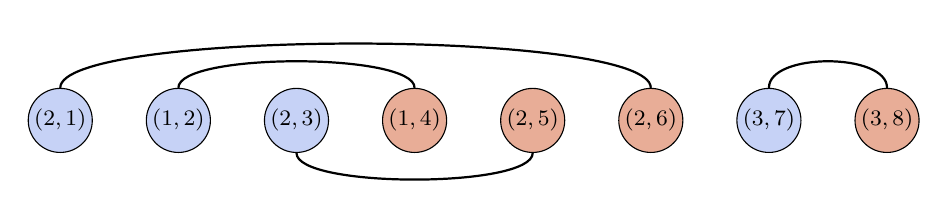
\begin{tikzpicture}[xscale=.5,yscale=.3,inner sep=1pt,node distance=1.5cm]
        \tikzstyle{Vertex}=[draw,circle,minimum size=.35cm,font=\footnotesize]
        \draw node[Vertex,fill=RoyalBlue!30](U01){$(2, 1)$};
        \draw node[Vertex,fill=RoyalBlue!30,right of=U01](U02) {$(1, 2)$};
        \draw node[Vertex,fill=RoyalBlue!30,right of=U02](U03){$(2, 3)$};
        \draw node [Vertex,fill=BrickRed!30,right of=U03](U04) {$(1, 4)$};
        \draw node [Vertex,fill=BrickRed!30,right of=U04](U05) {$(2, 5)$};
        \draw node [Vertex,fill=BrickRed!30,right of=U05](U06){$(2, 6)$};
        \draw node [Vertex,fill=RoyalBlue!30,right of=U06](U07){$(3, 7)$};
        \draw node [Vertex,fill=BrickRed!30,right of=U07](U08){$(3, 8)$};
        \draw [thick,>=latex']
        (U01.north) .. controls ($ (U01.north) + (0,2.5) $)
            and ($ (U06.north) + (0,2.5) $) .. (U06.north);
        \draw [thick,>=latex']
        (U02.north) .. controls ($ (U02.north) + (0,1.5) $)
            and ($ (U04.north) + (0,1.5) $) .. (U04.north);
        \draw [thick,>=latex']
        (U03.south) .. controls ($ (U03.south) + (0,-1.5) $)
            and ($ (U05.south) + (0,-1.5) $) .. (U05.south);
        \draw [thick,>=latex']
        (U07.north) .. controls ($ (U07.north) + (0,1.5) $)
            and ($ (U08.north) + (0,1.5) $) .. (U08.north);
    \end{tikzpicture}
    \end{split}\,.
    \end{equation*}
    \vspace{-1.5em}
\end{block}

\begin{block}{Definition}
    A perfect matching $(V, E)$ of a word $u$ is \alert{inclusion-free}
    if there are no edges $(u_i, i) \-- (u_j, j)$ and
    $(u_k, k) \-- (u_\ell, \ell)$ of $E$ such that $i < k < \ell < j$.
\end{block}
\end{frame}

%%%%%%%%%%%%%%%%%%%%%%%%%%%%%%%%%%%%%%%%%%%%%%%%%%%%%%%%%%%%%%%%%%%%%%%%
\begin{frame} \frametitle{Recognizing square words}

\begin{block}{Proposition \BIB{Rizzi, Vialette}{2013}}
    A word $u$ is a square iff $u$ admits an inclusion-free perfect
    matching.
\end{block}
%\medskip

\begin{block}{Example}
    The square word
    \begin{math}
        \textcolor{RoyalBlue}{3}\textcolor{BrickRed}{3}
        \textcolor{RoyalBlue}{12}\textcolor{BrickRed}{1}
        \textcolor{RoyalBlue}{2}\textcolor{BrickRed}{22}
    \end{math}
    admits the perfect matching \vspace{-1.5em}
    \begin{equation*}
        \begin{split}
        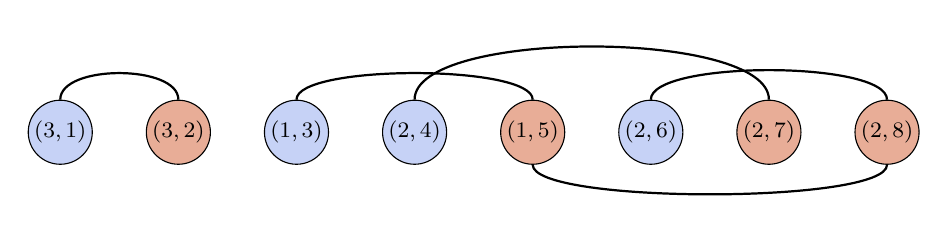
\begin{tikzpicture}[xscale=.5,yscale=.2,inner sep=1pt,node distance=1.5cm]
            \tikzstyle{Vertex}=[draw,circle,minimum size=.35cm,font=\footnotesize]
            \draw node[Vertex,fill=RoyalBlue!30](U01){$(3, 1)$};
            \draw node[Vertex,fill=BrickRed!30,right of=U01](U02) {$(3, 2)$};
            \draw node[Vertex,fill=RoyalBlue!30,right of=U02](U03){$(1, 3)$};
            \draw node[Vertex,fill=RoyalBlue!30,right of=U03](U04) {$(2, 4)$};
            \draw node[Vertex,fill=BrickRed!30,right of=U04](U05) {$(1, 5)$};
            \draw node[Vertex,fill=RoyalBlue!30,right of=U05](U06){$(2, 6)$};
            \draw node[Vertex,fill=BrickRed!30,right of=U06](U07){$(2, 7)$};
            \draw node[Vertex,fill=BrickRed!30,right of=U07](U08){$(2, 8)$};
            \draw [thick,>=latex']
            (U01.north) .. controls ($ (U01.north) + (0,2.25) $)
                and ($ (U02.north) + (0,2.25) $) .. (U02.north);
            \draw [thick,>=latex']
            (U03.north) .. controls ($ (U03.north) + (0,2.25) $)
                and ($ (U05.north) + (0,2.25) $) .. (U05.north);
            \draw [thick,>=latex']
            (U04.north) .. controls ($ (U04.north) + (0,4.5) $)
                and ($ (U07.north) + (0,4.5) $) .. (U07.north);
            \draw [thick,>=latex']
            (U05.south) .. controls ($ (U05.south) + (0,-2.5) $)
                and ($ (U08.south) + (0,-2.5) $) .. (U08.south);
            \draw [thick,>=latex']
            (U06.north) .. controls ($ (U06.north) + (0,2.5) $)
                and ($ (U08.north) + (0,2.5) $) .. (U08.north);
        \end{tikzpicture}
        \end{split}
    \end{equation*}

    \vspace{-1.5em}
    which is inclusion-free.
\end{block}
%\medskip

\begin{block}{Example}
    The word $1221$ is not a square. Its only perfect matching\vspace{-1.5em}
    \begin{equation*}
        \begin{split}
        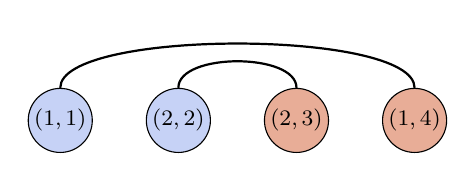
\begin{tikzpicture}[xscale=.5,yscale=.3,inner sep=1pt,node distance=1.5cm]
            \tikzstyle{Vertex}=[draw,circle,minimum size=.35cm,font=\footnotesize]
            \draw node[Vertex,fill=RoyalBlue!30](U01){$(1, 1)$};
            \draw node[Vertex,fill=RoyalBlue!30,right of=U01](U02) {$(2, 2)$};
            \draw node[Vertex,fill=BrickRed!30,right of=U02](U03){$(2, 3)$};
            \draw node [Vertex,fill=BrickRed!30,right of=U03](U04) {$(1, 4)$};
            \draw [thick,>=latex']
            (U01.north) .. controls ($ (U01.north) + (0,2.5) $)
                and ($ (U04.north) + (0,2.5) $) .. (U04.north);
            \draw [thick,>=latex']
            (U02.north) .. controls ($ (U02.north) + (0,1.5) $)
                and ($ (U03.north) + (0,1.5) $) .. (U03.north);
        \end{tikzpicture}\vspace{-1.5em}
        \end{split}
    \end{equation*}

    \vspace{-1.5em}
    is not inclusion-free.
\end{block}
\end{frame}

%%%%%%%%%%%%%%%%%%%%%%%%%%%%%%%%%%%%%%%%%%%%%%%%%%%%%o%%%%%%%%%%%%%%%%%%
\begin{frame} \frametitle{Main motivations}
Let $S_n$ be the set of permutations of size $n$.
\medskip

There are several products on permutations, analogs of the shuffle
product of words. Among these, there are
\smallskip

\begin{itemize}
    \item the shifted shuffle product \BIB{Duchamp, Hivert, Thibon}{2002};
    \medskip

    \item the convolution product \BIB{Duchamp, Hivert, Thibon}{2002};
    \medskip

    \item the supershuffle \BIB{Vargas}{2014}.
\end{itemize}
\medskip

\begin{block}{Main questions}
    \begin{itemize}
        \item How the previous key results about the shuffle of words
        translate for the supershuffle of permutations?
        \medskip

        \item
    \end{itemize}
\end{block}
\end{frame}

%%%%%%%%%%%%%%%%%%%%%%%%%%%%%%%%%%%%%%%%%%%%%%%%%%%%%%%%%%%%%%%%%%%%%%%%%%%%%%


%%%%%%%%%%%%%%%%%%%%%%%%%%%%%%%%%%%%%%%%%%%%%%%%%%%%%%%%%%%%%%%%%%%%%%%%
%%%%%%%%%%%%%%%%%%%%%%%%%%%%%%%%%%%%%%%%%%%%%%%%%%%%%%%%%%%%%%%%%%%%%%%%
%%%%%%%%%%%%%%%%%%%%%%%%%%%%%%%%%%%%%%%%%%%%%%%%%%%%%%%%%%%%%%%%%%%%%%%%
\section{Algebraic issues}

%%%%%%%%%%%%%%%%%%%%%%%%%%%%%%%%%%%%%%%%%%%%%%%%%%%%%%%%%%%%%%%%%%%%%%%%
\begin{frame} \frametitle{Combinatorial products and structure coefficients}
Let $C$ be a set of combinatorial objects and $\QQ[C]$ be the
$\QQ$-linear span of $C$.
\medskip

A binary linear product
\begin{equation*}
    \cdot : \QQ[C] \otimes \QQ[C] \to \QQ[C].
\end{equation*}
on $\QQ[C]$ describes a way to \alert{combine} two objects of
$C$ to obtain \alert{bigger} objects.
\medskip

In a general way, for any $x, y \in C$,
\begin{equation*}
    x \cdot y = \sum_{z \in C} \lambda_{x, y}^z \; z.
\end{equation*}
\medskip

A product is therefore wholly encoded by the coefficients
$\lambda_{x, y}^z \in \QQ$, $x, y, z \in C$, called
\alert{structure coefficients}.
\end{frame}

%%%%%%%%%%%%%%%%%%%%%%%%%%%%%%%%%%%%%%%%%%%%%%%%%%%%%%%%%%%%%%%%%%%%%%%%
\begin{frame} \frametitle{Combinatorial coproducts}
In a dual way, a linear coproduct
\begin{equation*}
    \Delta : \QQ[C] \to \QQ[C] \otimes \QQ[C].
\end{equation*}
on $\QQ[C]$ describe a way to \alert{break} one object of $C$ into
\alert{two smaller} pieces.
\medskip

In a general way, for any $z \in C$,
\begin{equation*}
    \Delta(z) = \sum_{x, y \in C}  \lambda_{x, y}^z \;  x \otimes y.
\end{equation*}
\medskip

A coproduct is therefore wholly encoded by the coefficients
$\lambda_{x, y}^z \in \QQ$, $x, y, z \in C$, called
\alert{structure coefficients}.
\end{frame}

%%%%%%%%%%%%%%%%%%%%%%%%%%%%%%%%%%%%%%%%%%%%%%%%%%%%%%%%%%%%%%%%%%%%%%%%
\begin{frame} \frametitle{Equivalence between products and coproducts}
\begin{block}{Key idea}
    Knowing how to break a combinatorial object is equivalent
    to knowing how to combine these.
\end{block}
\medskip

Indeed, if $\cdot : \QQ[C] \otimes \QQ[C] \to \QQ[C]$ is a product with
structure coefficients $\lambda_{x, y}^z \in \QQ$, $x, y, z \in C$,
we can define its \alert{dual coproduct} $\Delta$ by setting
\begin{equation*}
    \Delta(z) := \sum_{x, y \in C}  \lambda_{x, y}^z \;  x \otimes y.
\end{equation*}
\medskip

Conversely, if $\Delta : \QQ[C] \to \QQ[C] \otimes \QQ[C]$ is
a coproduct with structure coefficients $\lambda_{x, y}^z \in \QQ$,
$x, y, z \in C$, we can define its \alert{dual product} $\cdot$ by
setting
\begin{equation*}
    x \cdot y := \sum_{z \in C} \lambda_{x, y}^z \; z.
\end{equation*}
\end{frame}

%%%%%%%%%%%%%%%%%%%%%%%%%%%%%%%%%%%%%%%%%%%%%%%%%%%%%%%%%%%%%%%%%%%%%%%%
\begin{frame} \frametitle{Example: unshuffling binary words}
Let $B$ the set of all binary words and let us consider the coproduct
\begin{equation*}
    \Delta : \QQ[B] \to \QQ[B] \otimes \QQ[B]
\end{equation*}
on binary words defined by
\begin{equation*}
    \Delta(u) :=
    \sum_{P \sqcup Q = \{1, \dots, |u|\}}
    u_{|P} \otimes u_{|Q}.
\end{equation*}

\begin{block}{Example}
\begin{equation*}
    \Delta(100) =
    \epsilon \otimes 100 + 1 \otimes 00
    + 2 (0 \otimes 10) + 2 (10 \otimes 0) + 00 \otimes 1
    + 100 \otimes \epsilon
\end{equation*}
\end{block}
\end{frame}

%%%%%%%%%%%%%%%%%%%%%%%%%%%%%%%%%%%%%%%%%%%%%%%%%%%%%o%%%%%%%%%%%%%%%%%%
\begin{frame} \frametitle{Example: shuffling binary words}
\begin{block}{Proposition \BIB{Reutenauer}{1993}}
    The shuffle product of binary words is the dual product of the
    unshuffling coproduct of binary words.
\end{block}
\medskip

\begin{block}{Example}
Since
\begin{equation*}
    \textcolor{RoyalBlue}{\Delta(100)} =
    \epsilon \otimes 100 + 1 \otimes 00
    + \textcolor{Orange}{2} (\textcolor{BrickRed}{0 \otimes 10})
    + 2 (10 \otimes 0) + 00 \otimes 1
    + 100 \otimes \epsilon,
\end{equation*}
we observe that $\textcolor{BrickRed}{0 \otimes 10} $ has multiplicity
$\textcolor{Orange}{2}$ in $\textcolor{RoyalBlue}{\Delta(100)}$.
\medskip

By duality, this implies that $\textcolor{RoyalBlue}{100}$ has
multiplicity $\textcolor{Orange}{2}$ in
$\textcolor{BrickRed}{0 \shuffle 10}$. Indeed,
\begin{equation*}
    \textcolor{BrickRed}{0 \shuffle 10} =
    010 + \textcolor{Orange}{2} (\textcolor{RoyalBlue}{100}).
\end{equation*}
\end{block}
\end{frame}

%%%%%%%%%%%%%%%%%%%%%%%%%%%%%%%%%%%%%%%%%%%%%%%%%%%%%%%%%%%%%%%%%%%%%%%%
\begin{frame} \frametitle{Unshuffling permutations}
If $u$ is a word of integers without multiple occurrence of a same letter,
the \alert{standardized} $\STD(u)$ of $u$ is the unique permutation of
$S_{|u|}$ order-isomorphic to~$u$.

\begin{block}{Example}
\begin{equation*}
    \STD(82194) = 42153
\end{equation*}
\end{block}
\medskip

\begin{block}{Definition}
    The \alert{unshuffling coproduct of permutations} is the
    coproduct on $\QQ[S]$ defined by
    \begin{equation*}
        \Delta(\pi) =
        \sum_{P \sqcup Q = \{1, \dots, |\pi|\}}
        \STD\left(\pi_{|P}\right) \otimes \STD\left(\pi_{|Q}\right).
    \end{equation*}
\end{block}

\begin{block}{Example}
\begin{equation*}
    \Delta(213) =
    \epsilon \otimes 213 + 2 (1 \otimes 12) +
    1 \otimes 21 + 2 (12 \otimes 1) + 21 \otimes 1
    + 213 \otimes \epsilon
\end{equation*}
\end{block}
\end{frame}

%%%%%%%%%%%%%%%%%%%%%%%%%%%%%%%%%%%%%%%%%%%%%%%%%%%%%%%%%%%%%%%%%%%%%%%%
\begin{frame} \frametitle{Shuffling permutations}
\begin{block}{Definition}
    The \alert{shuffling product of permutations} (supershuffle) is the
    product $\SHUFFLE$ on $\QQ[S]$ defined as the dual product of the
    unshuffling product of permutations.
\end{block}
\medskip

\begin{block}{Proposition}
The permutations appearing in $\sigma \SHUFFLE \nu$ are exactly the
one obtained by shuffling two words $u$ and $v$ respectively
order-isomorphic to $\sigma$ and $\nu$.
\end{block}
\medskip

\begin{block}{Example}
\begin{equation*}\begin{split}
    12 \SHUFFLE 21 & =
    1243 + 1324 + 2 (1342) + 2 (1423) + 3 (1432) +
    2134 + 2 (2314) \\[.5em]
    & + 3 (2341) + 2413 + 2 (2431) + 2 (3124) + 3142 +
    3 (3214) + 2 (3241) \\[.5em]
    & + 3421 + 3 (4123) + 2 (4132) + 2 (4213) + 4231 + 4312
\end{split}\end{equation*}
\end{block}
\end{frame}

%%%%%%%%%%%%%%%%%%%%%%%%%%%%%%%%%%%%%%%%%%%%%%%%%%%%%%%%%%%%%%%%%%%%%%%%
\begin{frame} \frametitle{Square permutations}
\begin{block}{Definition}
    A permutation $\pi$ is a \alert{square} (w.r.t. the shuffle product
    $\SHUFFLE$) if there is $\sigma \in S$ such that $\pi$ appears in
    $\sigma \SHUFFLE \sigma$.
\end{block}
\medskip

By duality, $\pi$ is a square if there is $\sigma \in S$ such that
$\sigma \otimes \sigma$ appears in $\Delta(\pi)$.
\medskip

\begin{block}{Proposition}
    A permutation $\pi$ is a square iff $\pi$ can be obtained by
    shuffling two order-isomorphic words.
\end{block}
\medskip

\begin{block}{Example}
    The permutation
    \begin{math}
        \pi :=
        \textcolor{RoyalBlue}{25}\textcolor{BrickRed}{16}
        \textcolor{RoyalBlue}{7}\textcolor{BrickRed}{83}
        \textcolor{RoyalBlue}{4}
    \end{math}
    is square since $\pi$ can be obtained by shuffling
    $\textcolor{BrickRed}{1683}$ and $\textcolor{RoyalBlue}{2574}$
    and
    \begin{math}
        \STD(\textcolor{BrickRed}{1683})
        = \STD(\textcolor{RoyalBlue}{2574})
        = 1342
    \end{math}.
\end{block}
\end{frame}

%%%%%%%%%%%%%%%%%%%%%%%%%%%%%%%%%%%%%%%%%%%%%%%%%%%%%%%%%%%%%%%%%%%%%%%%
\begin{frame} \frametitle{Some properties of square permutations}
The first numbers of square permutations of size $2$ are
\begin{equation*}
    1, 2, 20, 504, 21032, 1293418.
\end{equation*}
%\medskip

\begin{block}{Proposition}
    Let $\pi$ be a square permutation and $\sigma$ be a square root of
    $\pi$. Then,
    \begin{enumerate}
        \item $\widetilde{\pi}$ is a square and
        $\widetilde{\sigma}$ is one of its square roots;
        \smallskip

        \item $\bar \pi$ is a square and $\bar \sigma$ is one of
        its square roots;
        \smallskip

        \item $\pi^{-1}$ is a square and $\sigma^{-1}$ is one of
        its square roots.
    \end{enumerate}
\end{block}
\medskip

\begin{block}{Proposition}
    The set of binary words of length $n$ that are square w.r.t.
    $\shuffle$ is in one-to-one correspondence with the set of
    square permutations of length $n$ avoiding the patterns
    $213$ and~$231$.
\end{block}
\end{frame}

%%%%%%%%%%%%%%%%%%%%%%%%%%%%%%%%%%%%%%%%%%%%%%%%%%%%%%%%%%%%%%%%%%%%%%%%
%%%%%%%%%%%%%%%%%%%%%%%%%%%%%%%%%%%%%%%%%%%%%%%%%%%%%%%%%%%%%%%%%%%%%%%%
%%%%%%%%%%%%%%%%%%%%%%%%%%%%%%%%%%%%%%%%%%%%%%%%%%%%%%%%%%%%%%%%%%%%%%%%
\section{Algorithmic issues}

%%%%%%%%%%%%%%%%%%%%%%%%%%%%%%%%%%%%%%%%%%%%%%%%%%%%%%%%%%%%%%%%%%%%%%%%%%%%%%

\begin{frame}
  \frametitle{Permutation pattern}

  \begin{definition}
    A permutation $\pi$ is said to \emph{contain} the permutation $\sigma$ if there
    exists a subsequence of (not necessarily consecutive) entries of $\pi$ that
    has the same relative order as $\sigma$, and in this case $\sigma$ is said
    to be a pattern of $\pi$, written $\sigma \leq \pi$.

    \medskip

    Otherwise, $\pi$ is said to \emph{avoid} the permutation $\sigma$.
  \end{definition}

  \medskip

  \begin{exampleblock}{Example}
    \begin{itemize}
      \item
        The permutation $\pi = 391867452$ contains the pattern $\sigma = 51342$,
        as can be seen in the highlighted subsequence of
        $\pi = 3\mathbf{91}8\mathbf{674}52$
        (or $\pi = 3\mathbf{91}8\mathbf{67}4\mathbf{5}2$ or
        $\pi = 3\mathbf{91}8\mathbf{67}45\mathbf{2}$ or
        $\pi = 3\mathbf{91}867\mathbf{452}$.)

      \item
       Since the permutation $\pi = 391867452$ contains no increasing subsequence
       of length four, $\pi$ avoids $1234$.
    \end{itemize}
  \end{exampleblock}

\end{frame}

%%%%%%%%%%%%%%%%%%%%%%%%%%%%%%%%%%%%%%%%%%%%%%%%%%%%%%%%%%%%%%%%%%%%%%%%%%%%%%

\begin{frame}
  \frametitle{Square permutation}

  \begin{definition}
    A permutation is said to be a \emph{square} if it can be obtained by
    shuffling two order-isomorphic patterns
  \end{definition}

  \medskip

  \begin{exampleblock}{Example}
    \begin{itemize}
      \item
        The permutation $\pi = 25167834$ is a square since it can obtained by
        shuffling two order-isomorphic (\emph{i.e.} $1342$)
        patterns $1683$ and $2574$ as can be seen in the highlighted subsequence of
        $\pi = \mathbf{25}16\mathbf{7}83\mathbf{4}$.

      \medskip

      \item
       $\pi = 4123$ and $1432$ are not squares.
    \end{itemize}
  \end{exampleblock}

\end{frame}

%%%%%%%%%%%%%%%%%%%%%%%%%%%%%%%%%%%%%%%%%%%%%%%%%%%%%%%%%%%%%%%%%%%%%%%%%%%%%%

\begin{frame}
  \frametitle{Hardness}
  \framesubtitle{Oriented perfect matching}

  \begin{definition}[Property $\mathbf{P_1}$]
    Let $\pi$ be a permutation. An oriented perfect matching $\mathcal{M}$
    on $\pi$ is said to have property $\mathbf{P_1}$ if it avoids all the
    six patterns \InclusionLL, \InclusionLR, \InclusionRL,
    \InclusionRR, \CrossingLR, and \CrossingRL.
  \end{definition}

  \medskip

  \begin{definition}[Property $\mathbf{P_2}$]
    Let $\pi$ be a permutation. An oriented perfect matching $\mathcal{M}$
    on $\pi$ is said to have property $\mathbf{P_2}$ if, for any two
    distinct arcs $(\pi(a), \pi(a'))$ and $(\pi(b), \pi(b'))$ in $\mathcal{M}$,
    we have $\pi(a) < \pi(b)$ if and only if $\pi(a') < \pi(b')$.
  \end{definition}
\end{frame}

%%%%%%%%%%%%%%%%%%%%%%%%%%%%%%%%%%%%%%%%%%%%%%%%%%%%%%%%%%%%%%%%%%%%%%%%%%%%%%

\begin{frame}
  \frametitle{Hardness}
  \framesubtitle{Oriented perfect matching}

  \begin{theorem}
    Let $\pi$ be a permutation. The following statements are equivalent:
    \begin{enumerate}
      \item The permutation $\pi$ is a square.
      \item There exists an oriented perfect matching $\mathcal{M}$
      on $\pi$ satisfying~$\mathbf{P_1}$ and~$\mathbf{P_2}$.
    \end{enumerate}
  \end{theorem}

  \medskip

  \onslide<2->
  \begin{exampleblock}{Example}
    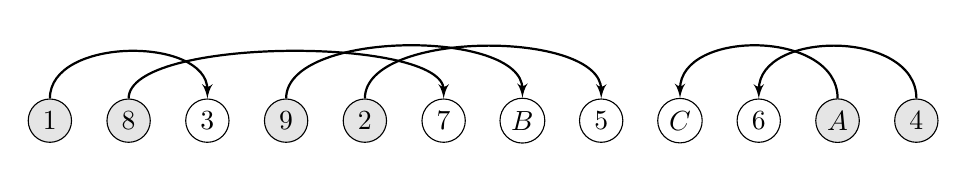
\begin{tikzpicture}[scale=0.35,inner sep=2pt,node distance=1cm]
        \draw node [draw,circle,minimum size=.55cm,fill=black!10](U01){$1$};
        \draw node [draw,circle,minimum size=.55cm,fill=black!10,right of=U01]
            (U02) {$8$};
        \draw node [draw,circle,minimum size=.55cm,right of=U02](U03){$3$};
        \draw node [draw,circle,minimum size=.55cm,fill=black!10,right of=U03]
            (U04) {$9$};
        \draw node [draw,circle,minimum size=.55cm,fill=black!10,right of=U04]
            (U05) {$2$};
        \draw node [draw,circle,minimum size=.55cm,right of=U05](U06){$7$};
        \draw node [draw,circle,minimum size=.55cm,right of=U06](U07){$B$};
        \draw node [draw,circle,minimum size=.55cm,right of=U07](U08){$5$};
        \draw node [draw,circle,minimum size=.55cm,right of=U08](U09){$C$};
        \draw node [draw,circle,minimum size=.55cm,right of=U09](U10){$6$};
        \draw node [draw,circle,minimum size=.55cm,fill=black!10,right of=U10]
            (U11) {$A$};
        \draw node [draw,circle,minimum size=.55cm,fill=black!10,right of=U11]
            (U12) {$4$};
        \draw [thick,->,>=latex']
        (U01.north) .. controls ($ (U01.north) + (0,2.25) $)
            and ($ (U03.north) + (0,2.25) $) .. (U03.north);
        \draw [thick,->,>=latex']
        (U02.north) .. controls ($ (U02.north) + (0,2.25) $)
            and ($ (U06.north) + (0,2.25) $) .. (U06.north);
        \draw [thick,->,>=latex']
        (U04.north) .. controls ($ (U04.north) + (0,2.5) $)
            and ($ (U07.north) + (0,2.5) $) .. (U07.north);
        \draw [thick,->,>=latex']
        (U05.north) .. controls ($ (U05.north) + (0,2.5) $)
            and ($ (U08.north) + (0,2.5) $) .. (U08.north);
        \draw [thick,->,>=latex']
        (U11.north) .. controls ($ (U11.north) + (0,2.5) $)
            and ($ (U09.north) + (0,2.5) $) .. (U09.north);
        \draw [thick,->,>=latex']
        (U12.north) .. controls ($ (U12.north) + (0,2.5) $)
            and ($ (U10.north) + (0,2.5) $) .. (U10.north);
    \end{tikzpicture}

    {\small%
    An oriented perfect matching $\mathcal{M}$ on the permutation
    $\pi = 183927B5C6A4$ satisfying the properties $\mathbf{P_1}$
    and $\mathbf{P_2}$. From $\mathcal{M}$, it follows that $\pi$ is
    a square as it appears in the shuffle of $1892A4$ and $37B5C6$,
    both being order-isomorphic to $145263$.
    }%end small
  \end{exampleblock}
\end{frame}

%%%%%%%%%%%%%%%%%%%%%%%%%%%%%%%%%%%%%%%%%%%%%%%%%%%%%%%%%%%%%%%%%%%%%%%%%%%%%%

\begin{frame}
  \frametitle{Hardness}

  \begin{theorem}
    Deciding whether a permutation is a square is \NPC.
  \end{theorem}

  \medskip

  \begin{block}{Remarks}
    \begin{itemize}
      \item
      We reduce from the problem of deciding wether a pattern $\sigma$ occurs in a
      permutation $\pi$.

      \smallskip

      \item
      Construct a new permutation $\mu$ such that
      $\sigma$ occurs in $\pi$ if and only if
      there exists an oriented perfect matching $\mathcal{M}$ on $\mu$
      satisfying $\mathbf{P_1}$ and $\mathbf{P_2}$.
    \end{itemize}
  \end{block}
\end{frame}

%%%%%%%%%%%%%%%%%%%%%%%%%%%%%%%%%%%%%%%%%%%%%%%%%%%%%%%%%%%%%%%%%%%%%%%%%%%%%%

\begin{frame}
  \frametitle{Hardness}

  \centering
  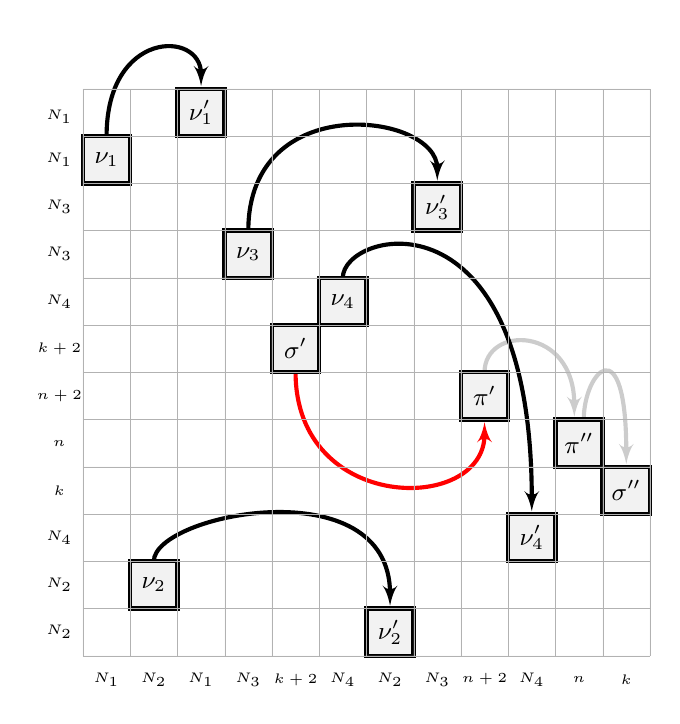
\begin{tikzpicture}[
    scale=.6,
    >=stealth',
    shorten >=1pt,
    main node/.style={align=center},
    cell/.style={draw,ultra thick,fill=black!5},
    structure link/.style={line width=1.5pt},
    pattern link/.style={line width=1.5pt,black!20},
    monotone/.style={draw,ultra thick,fill=black!5}
    ]
    % arcs
    % pi 1 - pi 2
    \draw [pattern link,->,>=latex'] (8.5,6) .. controls +(0,1) and +(0,2) .. (10.4,5);
    % pi 2 - sigma 2
    \draw [pattern link,->,>=latex'] (10.6,5) .. controls +(0,1) and +(0,3) .. (11.5,4);
    % 1
    \draw [structure link,->,>=latex'] (0.5,11) .. controls +(0,2.25) and +(0,1.25) .. (2.5,12);
    % 2
    \draw [structure link,->,>=latex'] (1.5,2) .. controls +(0,1) and +(0,3) .. (6.5,1);
    % 3
    \draw [structure link,->,>=latex'] (3.5,9) .. controls +(0,3) and +(0,1.5) .. (7.5,10);
    % 4
    \draw [structure link,->,>=latex'] (5.5,8) .. controls +(0,1) and +(0,7) .. (9.5,3);
    % sigma 1 - pi 1
    \draw [structure link,->,>=latex',red] (4.5,6) .. controls +(0,-3) and +(0,-2) .. (8.5,5);
    % nodes
    % 1
    \draw [cell] (0,10) -- (1,10) -- (1,11) -- (0,11) -- cycle;
    \draw [monotone] (0.5,10.5) node {\small  $\nu_1$};
    \draw [cell] (2,11) -- (3,11) -- (3,12) -- (2,12) -- cycle;
    \draw [monotone] (2.5,11.5) node {\small  $\nu'_1$};
    % 2
    \draw [cell] (1,1) -- (2,1) -- (2,2) -- (1,2) -- cycle;
    \draw [monotone] (1.5,1.5) node {\small  $\nu_2$};
    \draw [cell] (6,0) -- (7,0) -- (7,1) -- (6,1) -- cycle;
    \draw [monotone] (6.5,0.5) node {\small  $\nu'_2$};
    % 3
    \draw [cell] (3,8) -- (4,8) -- (4,9) -- (3,9) -- cycle;
    \draw [monotone] (3.5,8.5) node {\small  $\nu_3$};
    \draw [cell] (7,9) -- (8,9) -- (8,10) -- (7,10) -- cycle;
    \draw [monotone] (7.5,9.5) node {\small  $\nu'_3$};
    % 4
    \draw [cell] (5,7) -- (6,7) -- (6,8) -- (5,8) -- cycle;
    \draw [monotone] (5.5,7.5) node {\small $\nu_4$};
    \draw [cell] (9,2) -- (10,2) -- (10,3) -- (9,3) -- cycle;
    \draw [monotone] (9.5,2.5) node {\small  $\nu'_4$};
    % sigma 1
    \draw [cell] (4,6) -- (5,6) -- (5,7) -- (4,7) -- cycle;
    \node [main node] (sigma1) at (4.5,6.5) {\small $\sigma'$};
    % pi 1
    \draw [cell] (8,5) -- (9,5) -- (9,6) -- (8,6) -- cycle;
    \node [main node] (pi1) at (8.5,5.5) {\small $\pi'$};
    % pi 2
    \draw [cell] (10,4) -- (11,4) -- (11,5) -- (10,5) -- cycle;
    \node [main node] (sigma2) at (10.5,4.5) {\small $\pi''$};
    % sigma 2
    \draw [cell] (11,3) -- (12,3) -- (12,4) -- (11,4) -- cycle;
    \node [main node] (pi2) at (11.5,3.5) {\small $\sigma''$};
    % grid
    \draw[step=1cm,black!30,ultra thin,fill=black!10] (0,0) grid (12,12);
    % row size
    \foreach \y/\N in {0.5/N_2,1.5/N_2,2.5/N_4,3.5/k,4.5/n,5.5/n+2,6.5/k+2,7.5/N_4,8.5/N_3,9.5/N_3,10.5/N_1,11.4/N_1} {
        \node at (-0.5,\y) (R\y) {\tiny $\N$};
    }
    % column size
    \foreach \x/\N in
    {0.5/N_1,1.5/N_2,2.5/N_1,3.5/N_3,4.5/k+2,5.5/N_4,6.5/N_2,7.5/N_3,8.5/n+2,9.5/N_4,10.5/n,11.5/k} {
        \node at (\x,-0.5) (C\x) {\tiny $\N$};
    }
  \end{tikzpicture}
\end{frame}

%%%%%%%%%%%%%%%%%%%%%%%%%%%%%%%%%%%%%%%%%%%%%%%%%%%%%%%%%%%%%%%%%%%%%%%%%%%%%%

\begin{frame}
  \frametitle{Open problems}

  \begin{block}{Combinatorics}
    How many permutations of length $2n$ are squares?

    \smallskip

    How many $(213,231)$-avoiding
    permutations of length $2n$ are squares? (Equivalently,
    how many binary strings of length $2n$ are squares?)
  \end{block}

  \medskip

  \begin{block}{Combinatorics}
    Given two permutations $\pi$ and~$\sigma$, how hard is the problem of
    deciding whether $\sigma$ is a square root of~$\pi$?
  \end{block}

  \medskip

  \begin{block}{Algebra}
    \ldots
  \end{block}

\end{frame}

%%%%%%%%%%%%%%%%%%%%%%%%%%%%%%%%%%%%%%%%%%%%%%%%%%%%%%%%%%%%%%%%%%%%%%%%%%%%%%

\end{document}
